\documentclass{article}
\usepackage{algpseudocode}
\usepackage[ruled]{algorithm}
\usepackage{url}
\usepackage{framed}
\usepackage{amsfonts,amsmath,amsthm,amssymb}
\usepackage{graphicx}
\usepackage{url}
\usepackage{color}
\usepackage{geometry}

\geometry{margin=1.2in}

\newcommand {\mean} {\ensuremath {\mathop{\mathrm{mean}}}}
\newcommand {\median} {\ensuremath {\mathop{\mathrm{median}}}}
\newcommand {\N} {\ensuremath {\mathcal{N}}}
\newcommand {\IE} {\ensuremath {\mathbb{E}}}
\newcommand {\cov} {\ensuremath {\mathop{\mathrm{cov}}}}
\newcommand {\BEL} {\ensuremath {\mathop{\mathrm{BEL}}}}

\newtheorem{lemma}{Lemma}

\title{VOI-aware Monte Carlo Sampling in Trees}
\author {David Tolpin, Solomon Eyal Shimony \\
Department of Computer Science, \\
Ben-Gurion University of the Negev, Beer Sheva, Israel \\
\{tolpin,shimony\}@cs.bgu.ac.il}

\begin{document}

\maketitle

\begin{abstract}
Upper bounds for the VOI are provided for pure exploration in the
Multi-armed Bandit Problem. Sampling policies based on the upper
bounds are suggested. Empirical evaluation of the policies is provided
on random problems as well on the Go game.
\end{abstract}

\section{Empirical Evaluation}

\begin{figure}[h]
\centering
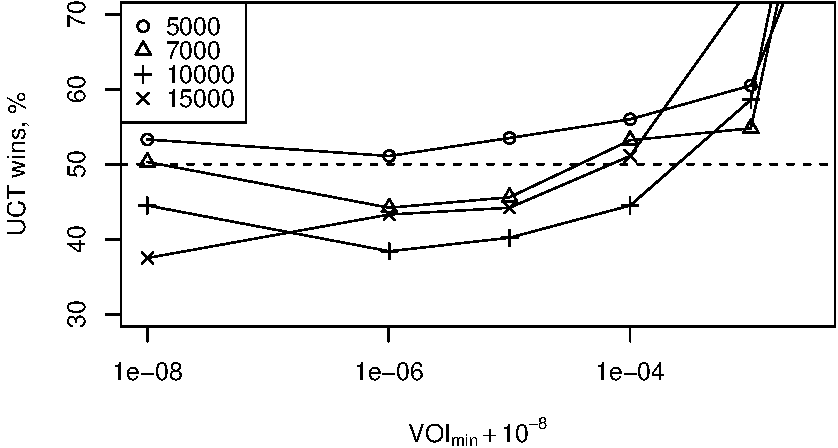
\includegraphics[scale=0.8]{vct-wins.pdf}
\caption{Winning rate: UCT against VCT}
\label{fig:uct-against-vct}
\end{figure}

\begin{figure}[h]
\centering
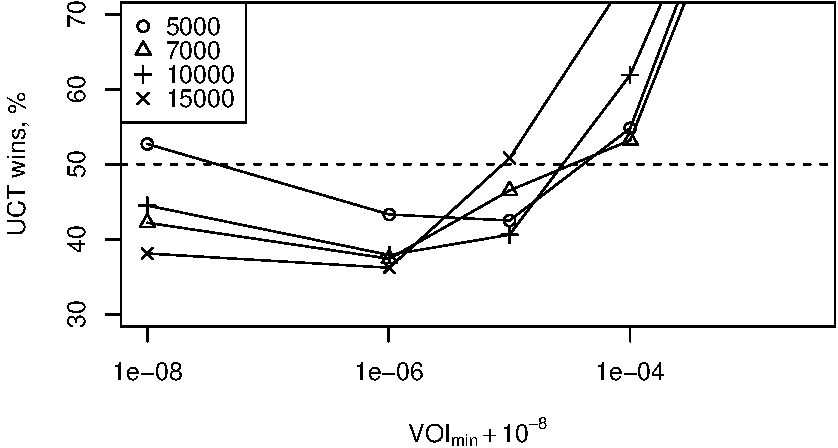
\includegraphics[scale=0.8]{ect-wins.pdf}
\caption{Winning rate: UCT against ECT}
\label{fig:uct-against-ect}
\end{figure}

\begin{figure}[h]
\centering
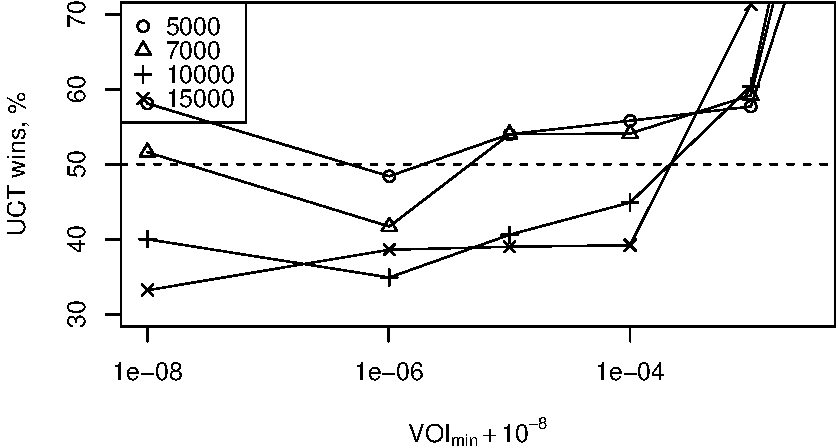
\includegraphics[scale=0.8]{bct-wins.pdf}
\caption{Winning rate: UCT against BCT}
\label{fig:uct-against-ect}
\end{figure}

\begin{figure}[h]
\centering
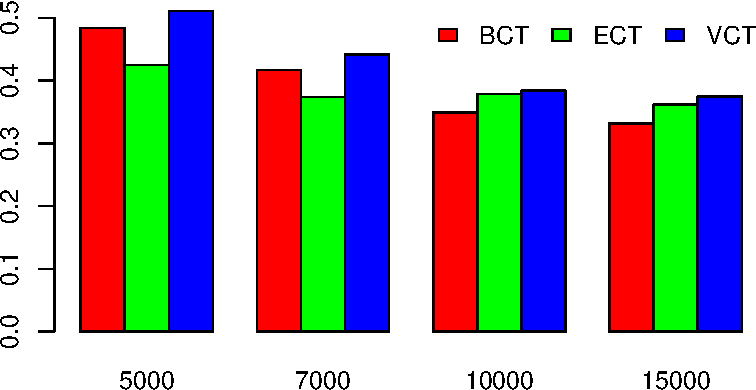
\includegraphics[scale=0.8]{bests-colorful.pdf}
\caption{Best winning rate comparison}
\label{fig:best-winning-rate}
\end{figure}

\clearpage


\bibliographystyle{plain}
\bibliography{refs}

\end{document}
